% mainfile: ../main.tex
\section{Introduction}
This chapter was published in the 20th ACM SIGKDD international
conference on Knowledge discovery and data mining (KDD 2014)~\cite{jin2014misinformation}.

In recent years social networking sites such as Twitter and Facebook have
provided not just a platform for communication but also a means
of mobilization and strategic interaction between key players
of social movements, e.g., protests. Traditionally social movements occur
within a subset of the population and have spread through on-the-ground
communities and unions. With the advent of leaner communication
technologies like Twitter, the way such movements form and
spread through modern society has changed. With Twitter, in particular,
traditional slogans have transformed into hashtags which can
offer a consistent way of communicating the reason and
motivation of social movements like protests and uprisings.

\begin{figure}[h]
\centering
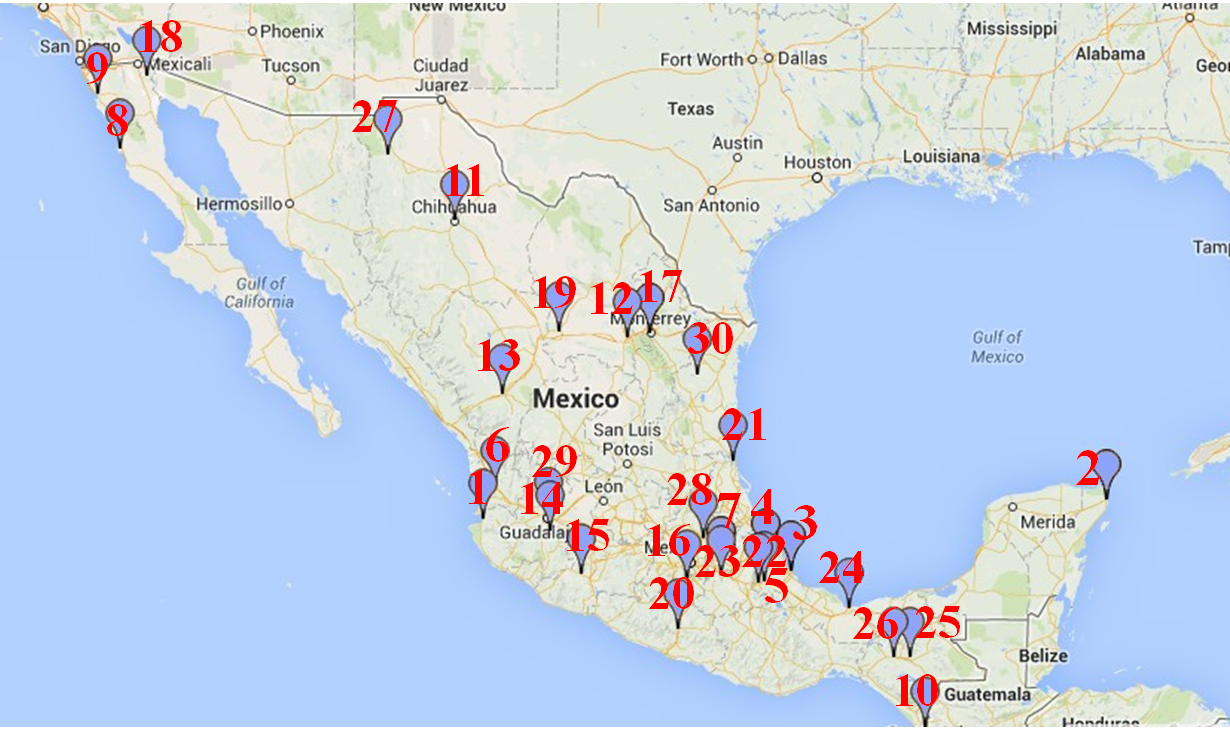
\includegraphics[scale=0.4]{figures/mexico_teacher_protest.png}
\caption{Mexico teacher protest events from Sep 1 to Sep 7, 2013. The blue pins denote protest cities; the numbers in red denote the sequence of
protests as they spread across the country.}
\label{fig:mexico_teacher}
\end{figure}


In this chapter, we focus on Twitter's
user networks during protests
and similar civil unrest activities in Latin America. Our goals
are to model the propagation and growth of contagion-like protest
waves within a social network and to understand the social and
structural dynamics underlying such phenomena. The key problem
is understanding the nature of information propagation among motivated
users of a social network. We have observed that such mass
protests emerge very swiftly and sharply. In Twitterspeak, they
would be considered trending but most such trends quickly decline
on the social network even if not in the physical world. Modeling
protest-related topic propagation on networks involves several challenges.

First, social protest propagation through online media can spread
over large areas more quickly than traditional
methods since users are geographically distributed. For example,
on September 1, 2013, the Mexican government's education reform bill drew
the wrath of teachers country-wide who opposed the reform
(which required regular assessments of their performance as educators).
Twitter was a virtual loudspeaker, providing a platform for organization
and strategization for teachers to put forth their arguments against
the bill. A series of mass teacher protests erupted and spread
from city to city. As shown in Fig.~\ref{fig:mexico_teacher}, we
see the movement spreading over time to different locations with
no obvious visual mobilization pattern. The second challenge is
that Twitter's user network embodies many subgraphs based on
social ties which might afford different propagation rates due to
subgraph-specific structures.

Thus identifying how the cause of a protest is adopted by Twitter users and how mobilization happens in the underlying network is a difficult task.
To address this problem we present an integrated framework with new
theoretical models as well as empirical validation on real Twitter
data for actual protests witnessed in the recent past. Our key
contributions are:

\iffalse
We also focus on the role of community driven information propagation over this bispace. We use \textit{Geometric Brownian Motion} (GBM) and Poisson processes over the mentions network and latent space respectively to model information propagation during mass social movements. When the protest-related information propagation starts, it propagates over the two spaces independently and simultaneously. In the mention network space, the propagation process follows Geometric Brownian diffusion over the defined social network. In the latent space, we believe propagation will obey the Poisson distribution. We introduce a trust function $S_t$ and Brownian distance $d_{ij}$ between users to describe the information propagation mechanism of the mentions network. Suppose that some user $v_i$'s trust with user $v_j$ at time $t$ is $S^{ij}_t$ and the distance from user $v_i$ to user $v_j$ is $d_{ij}$. Only when $ln(S^{ij}_t)$ is no less than the distance $d_{ij}$ is $v_j$ infected by $v_i$.
%We propose that the trust function $S_t$ follows a dynamic geometric Brownian motion
%\begin{equation}\frac{\partial S_t}{S_t} = \mu {dt}+\sigma dW_t
%\end{equation}


In the latent space, we model the propagation as a Poisson distribution, believing that it is difficult to account for all the ways in which information may spread. For a given time interval $T_p$, the probability of infecting users is expressed as $Pr(x=k)=\frac{\lambda^k e^{-\lambda}}{k!}$ where $\lambda$ is the average number of infected users during that time interval $T_p$.
\vspace{2 mm}
\fi

\begin{itemize}
\item
We model the inherent heterogeneity in propagation using a
bispace model, comprised of the Twitter mentions network (where
both globally and locally influential neighbors contribute to a user's
recruitment) and a
latent space (where external exposure to protest-related information is
captured).
\item We focus on the role of community-driven information propagation
over the bispace model. We use geometric Brownian motion (GBM)
over the mentions network and Poisson processes over the latent space to model information propagation during mass social movements.
\item We illustrate the effectiveness of our approach in modeling several key mass protest adoption scenarios in multiple countries of Latin America, viz.
Argentina, Brazil,
Colombia,
Mexico,
Uruguay, and
Venezuela.

\end{itemize}

The rest of this chapter is organized as follows. Section 2 covers related work in the areas of social movements, information diffusion in networks, external influences, and Brownian motion. Section 3 proposes the geometric Brownian motion propagation mechanism. Section 4 introduces the bispace propagation model, especially the model of propagation in latent space. In Section 5, we
present our dataset and experimental setup,
followed by initial experimental findings. Section 6 discusses the
evaluation results for our approach followed by a brief discussion in
Section 7.
